\begin{figure}
    \centering
    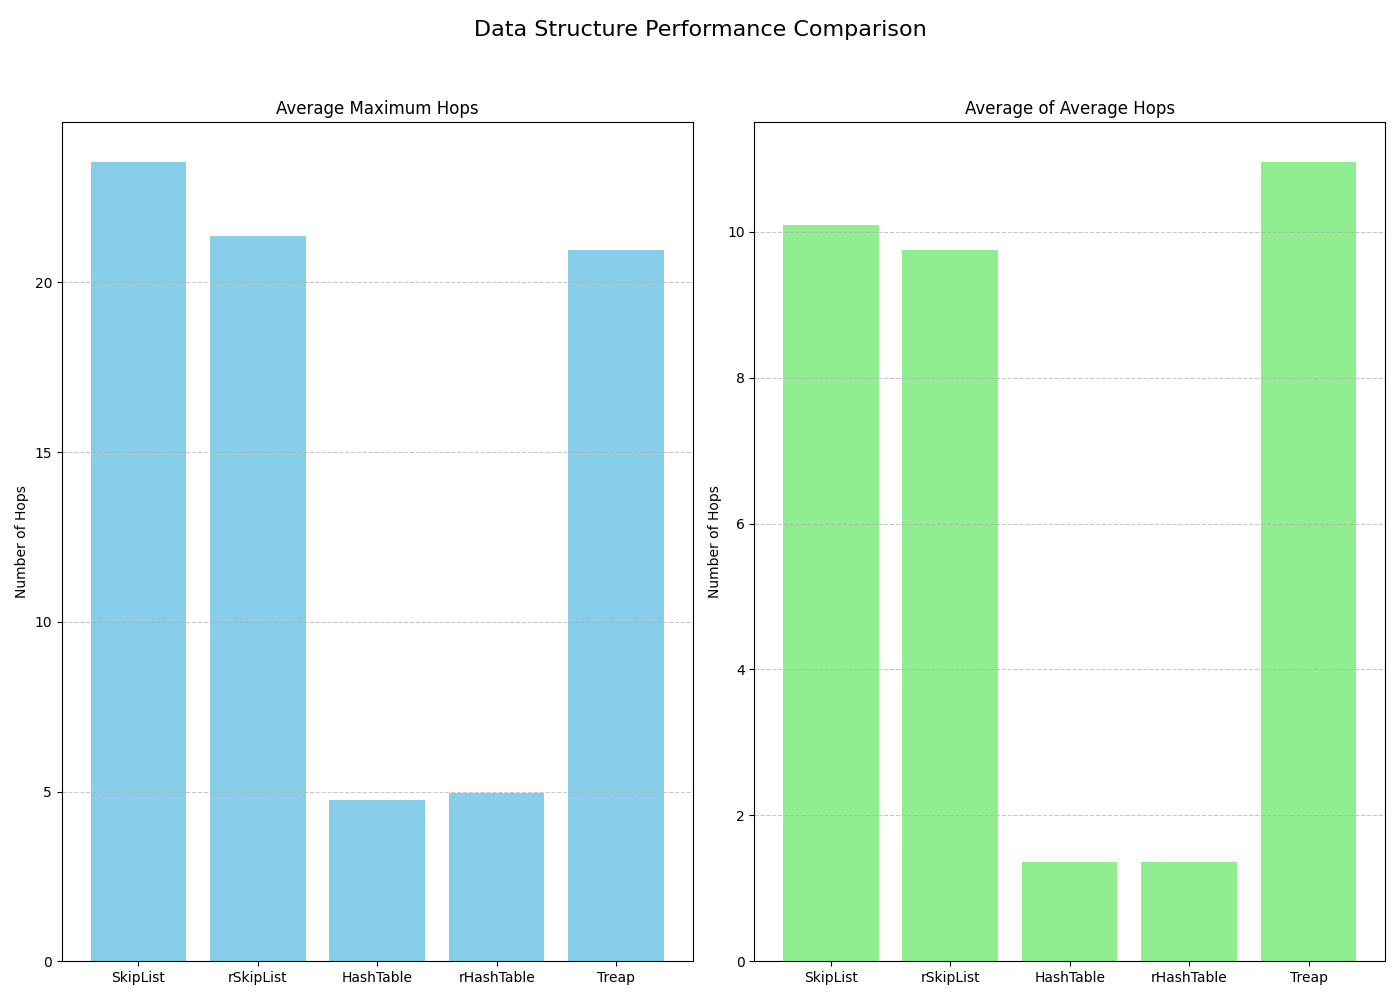
\includegraphics[width=\textwidth]{chapters/ch5_skipping/ch5_images/datastructure_performance.png}
    \caption[Non-adaptive PSDS Results.]{Maximum and average hop count in the non-adaptive setting, displayed on a linear scale.}
    \label{fig:runtimes_nonadaptive}
\end{figure}

\begin{figure}
    \centering
    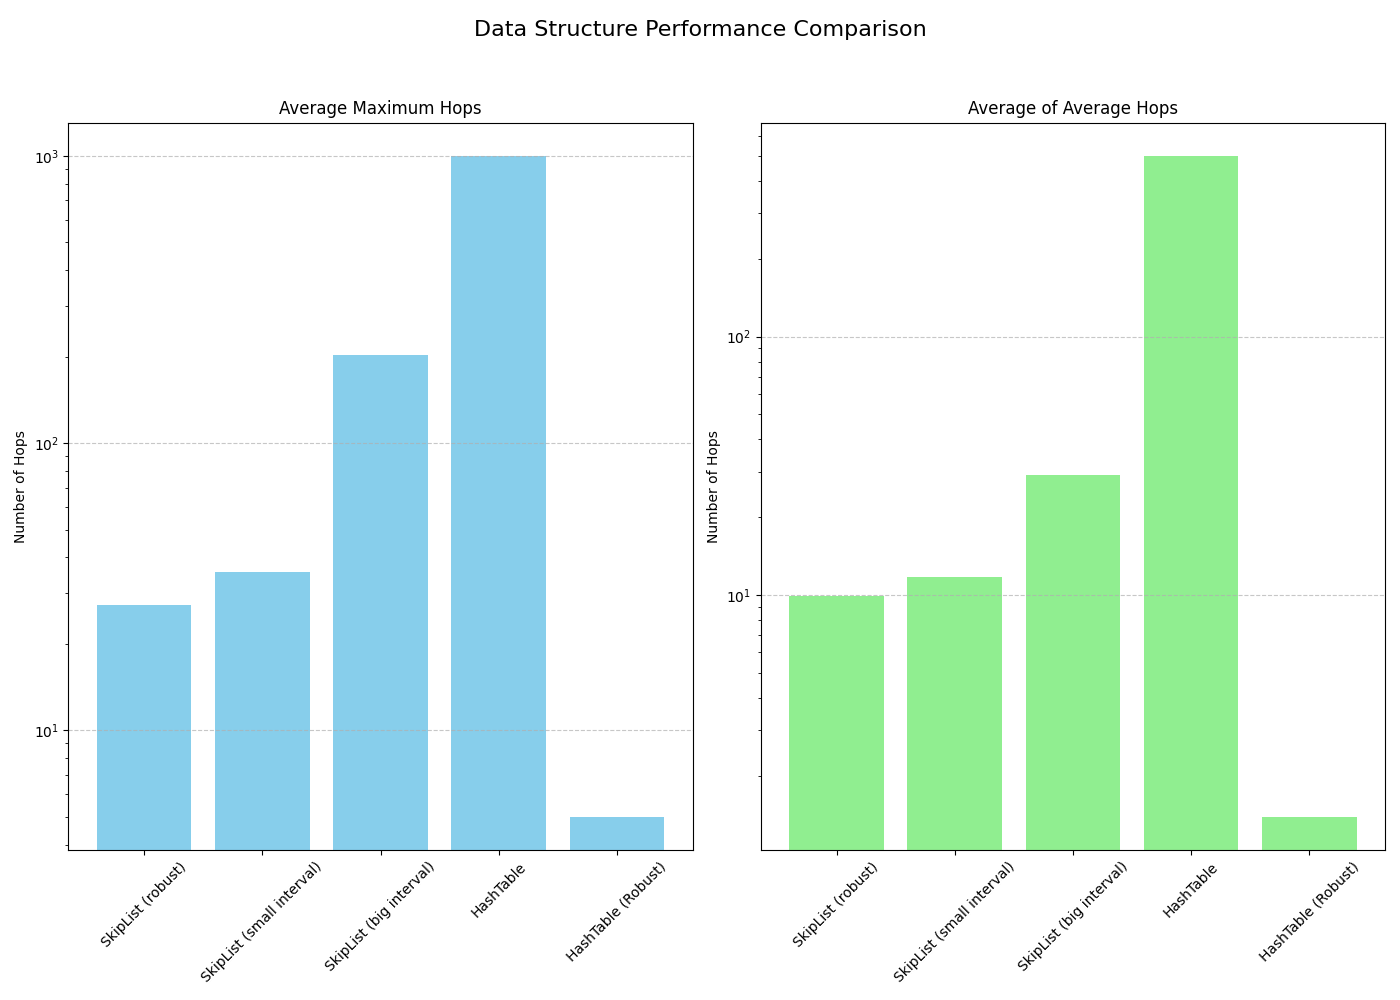
\includegraphics[width=\textwidth]{chapters/ch5_skipping/ch5_images/adaptive_datastructure_performance.png}
    \caption[Adaptive PSDS Results.]{Maximum and average hop count in the adaptive setting, displayed on a logarithmic scale.}
    \label{fig:runtimes_adaptive}
\end{figure}


We conducted experiments to empirically validate our analytical results. Our first experiment tested whether robust data structures offer benefits in non-adversarial settings. Using a dataset of 10 million usernames~\cite{10-mio}, we randomly inserted 1,000 usernames into each data structure. We measured performance by counting hops (forward movements between nodes). The hash table's load factor was limited to 0.7 \cite{mcclellan1974art}, and the skip list's maximum height was set to $log_{2} n$. We used Python's built-in hash function, which is vulnerable to multi-collision attacks. Results were averaged over 100 trials.

As shown in \Cref{fig:runtimes_nonadaptive}, the robust skip list consistently required fewer mean and maximum hops than its standard counterpart, demonstrating benefits even in non-adversarial settings with only constant overhead. The robust hash table showed comparable performance to the original structure. We benchmarked an unmodified treap implementation given its inherent adversarial robustness.

Our second experiment evaluated performance under adaptive adversarial conditions. We implemented a hash collision attack on hash tables and a gap attack on skip lists, averaging results over 100 trials. Treaps were excluded due to their established inherent robustness.

For the hash collision attack, we pre-calculated bucket values to deliberately insert all elements into a single bucket, creating worst-case conditions for standard hash tables. For the robust implementation, we used a random key for pre-calculation, since the actual secret key would be unknown to an attacker.

For the gap attack against skip lists, we tested two variants: a restricted version using the same username dataset and an unrestricted version using integers within the range $[0, 10^{100}]$\footnote{While this serves primarily as a proof of concept, such a vast interval could realistically be achieved using a 20-character limit with Unicode encoding. We emphasize that significant runtime degradation can be observed even with substantially smaller intervals.}. We report the top $1\%$ of outcomes with respect to the maximum hop count.

Results in~\Cref{fig:runtimes_adaptive} confirm that adversarial attacks significantly degrade standard implementations, while robust counterparts maintain consistent performance. The robust skip list maintained an average maximum hop count of 27.36, compared to 33.17 for the non-robust implementation under non-adaptive conditions. Under adaptive settings, the non-robust implementation degraded to 35.61 maximum average hops, and further to 202.71 hops when using the larger integer range. This validation confirms our theoretical findings on adversarial robustness, and also suggests that our remark regarding the artificial ``looseness'' of the bound carries weight.